\documentclass{article}


\usepackage{arxiv}

\usepackage[utf8]{inputenc} % allow utf-8 input
\usepackage{graphicx, multicol, latexsym, amsmath, amssymb}
\usepackage{blindtext}
\usepackage{subfigure}
\usepackage[T1]{fontenc}    % use 8-bit T1 fonts
\usepackage{hyperref}       % hyperlinks
\usepackage{url}            % simple URL typesetting
\usepackage{booktabs}       % professional-quality tables
\usepackage{amsfonts}       % blackboard math symbols
\usepackage{nicefrac}       % compact symbols for 1/2, etc.
\usepackage{microtype}      % microtypography
\usepackage{lipsum}
\usepackage[bottom]{footmisc}

\title{Diabetic Retinopathy Detection}


\author{
  Yitian Shi\\
 Electromobility\\
 University of Stuttgart\\
  Stuttgart 70569 \\
  \texttt{st175325@stud.uni-stuttgart.de} \\
  %% examples of more authors
   \And
Jonas Vogt\\
 Electromobility\\
 University of Stuttgart\\
  Stuttgart 70569 \\
  \texttt{st176729@stud.uni-stuttgart.de} \\
  %% \AND
  %% Coauthor \\
  %% Affiliation \\
  %% Address \\
  %% \texttt{email} \\
  %% \And
  %% Coauthor \\
  %% Affiliation \\
  %% Address \\
  %% \texttt{email} \\
  %% \And
  %% Coauthor \\
  %% Affiliation \\
  %% Address \\
  %% \texttt{email} \\
}

\begin{document}
\maketitle

\begin{abstract}
In this paper, we've tried different DNN architectures on the classification tasks (whether a patient has non-referable (NRDR) or referable diabetic retinopathy (RDR)) based on the Indian Diabetic Retinopathy Image Dataset (IDRID). The backbones of classifiers are such as ResNet, DenseNet, Inception, MobileNet, vision Transformer, etc., which are based on either random initialization or transfer learning. The highest test accuracy is 87.37\% for binary classification and 61.17\% for 5-class classification. Then we tried to visualize the training procedure by guided Grad-CAM at the same time. After that, we tuned the hyperparameters which mainly focus on the training procedure of vision Transformer 16 to achieve the best performance on the 5-class classification by using Weights\&Biases. Last but not least, we've also made some experiments on the Kaggle Dataset.

\end{abstract}


\section{Introduction}
Nowadays in medical image processing and analysis such as MRT diabetes diagnosis, one efficient and accurate approach is the utilization of end-to-end frameworks which are based on deep neural networks by analyzing retina pictures, which is gradually replacing the manual works. Furthermore, deep neural networks which can learn from small datasets to categorize medical images should be utilized to classify Diabetic Retinopathy, as this can be transferred to other medical image classification problems facing the challenge of insufficient training data\cite{misgina}.

Our experiments are based on the analysis of different common architectures as follows: In the section \ref{sec:dataset}, we'll briefly have an overview of the dataset and introduce our preprocessing pipeline. Then we'll give the results of all the highest balanced test accuracy including hard voting from different models and a deep visualization example in the section \ref{sec:model}. Furthermore, the detailed utilization of Weights\&Biases and the results of the 5-class classification will also be explained. In the section \ref{sec:conclusion}, we'll make our conclusion based on all the experiments and briefly talk about the Kaggle dataset.


\section{Dataset overview and preprocessing pipeline}
\label{sec:dataset}

\subsection{Dataset statistics (Jonas Vogt)}
In Figure \ref{fig:fig1} we can discover our difficulties from the distribution of labels, i.e. the unbalance of different labels and the Insufficiency of total data amount for training. To deal with these problems we require random oversampling to increase the amount of rare data. Meanwhile, data augmentation is necessary, which increases the variety of data and ensures the generalization and robustness of models.
\begin{figure}
\centering
{
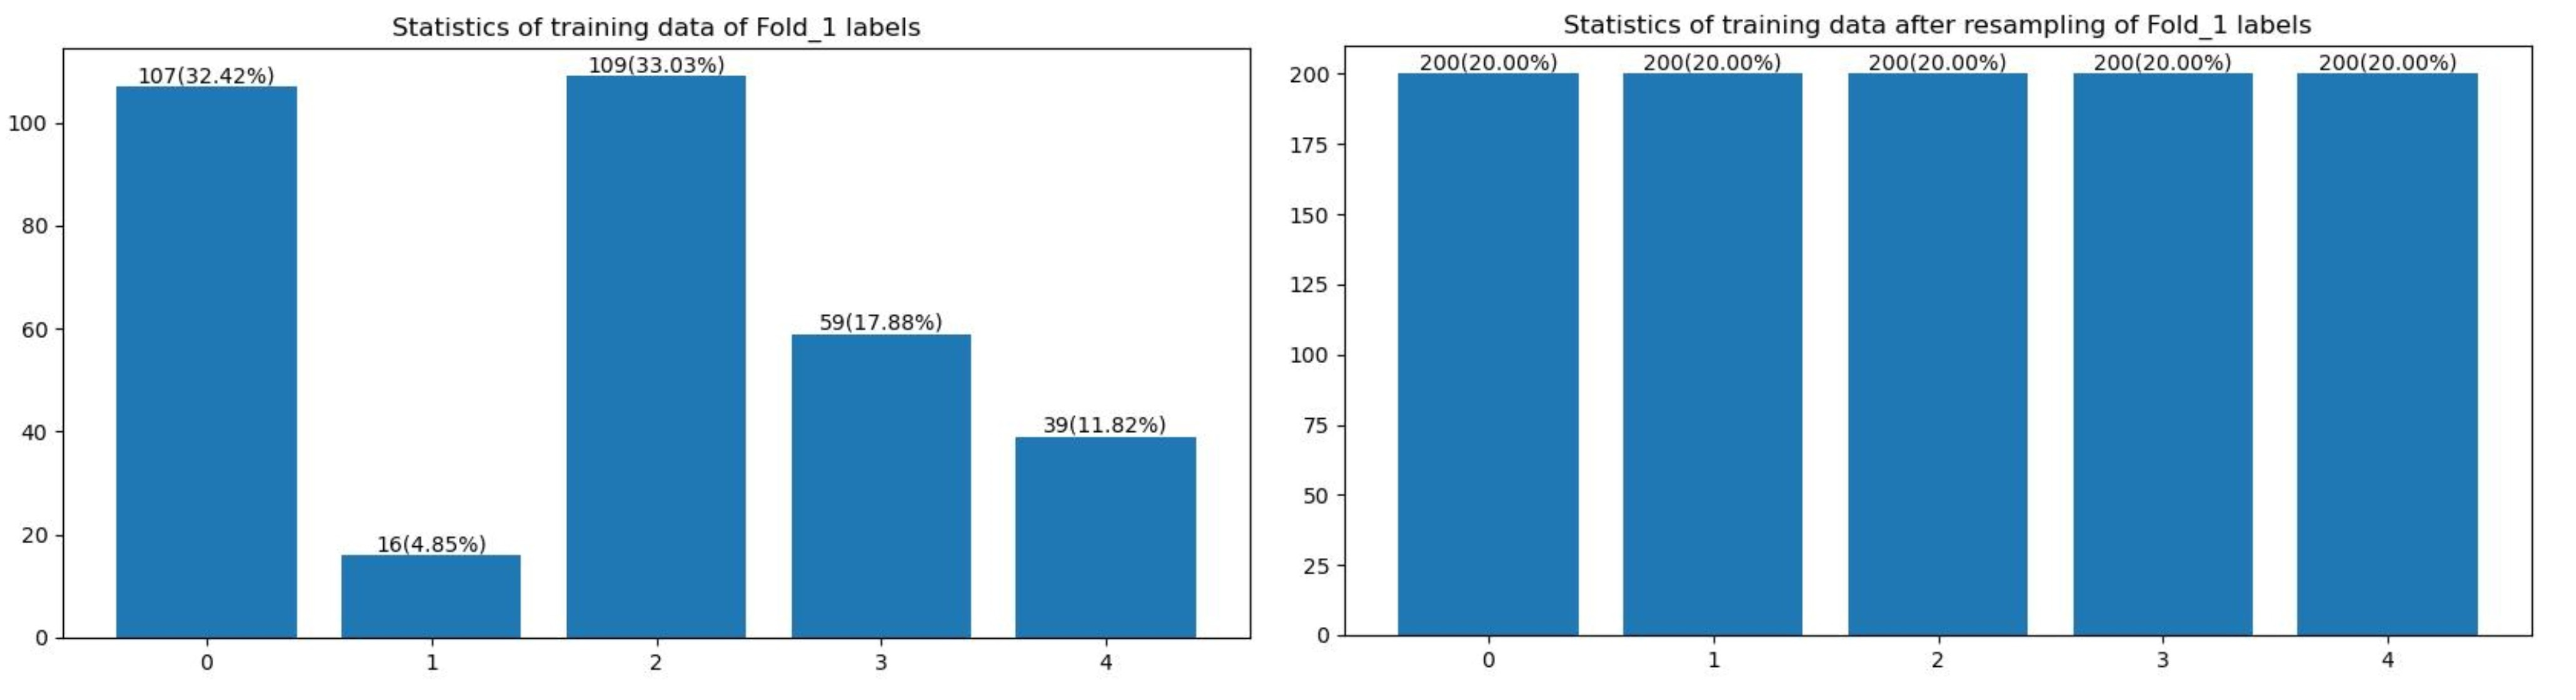
\includegraphics[scale=0.15]{../pictures/statistics/5-class-paper.png}
%\caption{fig1}
}
\caption{Dataset statistics}
\label{fig:fig1}
\end{figure}

\subsection{Data preprocessing (Yitian Shi)}
Before the data augmentation mentioned above, we should do some preprocessing, such as cropping and padding to our pictures, in which way the most relevant part of images will be easily captured in the model (Figure \ref{fig:fig2} middle). We've also built another pipeline, i.e. the Graham preprocessing, and tried to analyze its performance as well (Figure \ref{fig:fig2} right). Then, the data augmentation of pictures such as random shifting, rotation, scaling, resizing, brightness will be used (see Figure \ref{fig:fig3}).

Although this procedure can also be implemented in the TFRecord pipeline just like data augmentation, it's much more time-consuming. Therefore it will be finished at first and the preprocessed pictures will be saved as an independent dataset, which will be read by the parse function later on.
\begin{figure}
\centering
{
\includegraphics[scale=0.055]{../pictures/preprocessing example/preprocessing example.png}
%\caption{fig1}
}
\caption{Image preprocessing example}
\label{fig:fig2}
\end{figure}
\begin{figure}
\centering
{
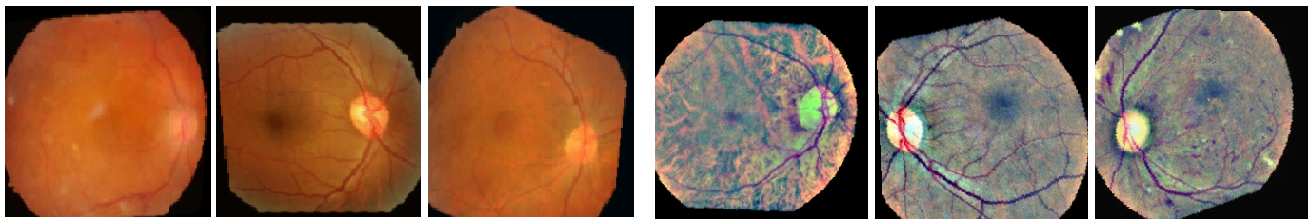
\includegraphics[scale=0.5]{../pictures/preprocessing example/augmentation.png}
%\caption{fig1}
}
\caption{Data augmentation}
\label{fig:fig3}
\end{figure}

\subsection{Stratified k-fold data generator (Yitian Shi)}
It's also worth mentioning that to deal with the Insufficiency of data and analyze the model architectures more comprehensively, we choose to use stratified k-fold cross-validation instead of training only once. For example, for a 5-fold training 20\% of data from each class label will be divided out as part of the validation set, and the training procedure will be repeated by 5 times. At last, we pick the model with the best test accuracy from those 5 models. 

\section{Models, results and matrics}
\label{sec:model}

\subsection{Binary classification (Jonas Vogt, Yitian Shi)}
The Results of all the best test accuracy we can achieve are as in Table \ref{tab:table1}. We've also computed the sensitivity, specificity, precision, etc. as our matrices. Some of the architectures used the dataset after Graham preprocessing which are remarked in the table. As we can see, the accuracy of models trained by those datasets can have around 1\% of improvement compared to some architecture with the original dataset. Note that some of the architectures are based on the pre-trained models by transfer learning.

\subsubsection{Ensemble learning (Jonas Vogt)}
Note that the last architecture, i.e. the hard voting in the table is based on the 5 architectures above (MobileNetV2, InceptionV3, EfficientnetB2, DenseNet121, and InceptionResNetV2), which gives us the best accuracy of 87.37\%.

\begin{table}
\caption{Results of different architectures}
\begin{tabular}{cccccccc}
\toprule
Architecture\footnote{}\	&Sensitivity	&Specificity	&Precision&	Accuracy	&Balanced accuracy	&F1 score \\
\midrule
ResNet18	&78.12\% &	94.87\%	&96.15\%	&84.46\%	&86.49\%	&86.21\%\\
ResNet34	&79.69\%	&92.31\%	&94.44\%	&84.46\%	&85.00\%	&86.44\%\\
ResNet34 (Graham) 	&87.50\%	&84.62\%	&90.32\%	&86.41\%	&86.06\%	&88.89\%	\\
ResNet50	&79.69\%	&97.44\%	&98.08\%	&86.40\%	&83.55\%	&87.93\%\\
MobileNetV2*	&76.56\%	&92.31\%	&94.23\%	&82.52\%	&84.44\%	&84.48\%\\
MobileNetV2* (Graham)	&87.50\%	&79.49\%	&87.50\%	&84.47\%	&83.49\%	&87.50\%	\\
InceptionV3*	&84.38\%	&84.62\%	&90.00\%	&84.47\%	&84.50\%	&87.10\%\\
InceptionResNetV2*	&76.56\%	&92.31\%	&94.23\%	&82.52\%	&84.44\%	&84.48\%\\
DenseNet121*	&84.38\%	&79.49\%	&87.10\%	&82.51\%	&81.92\%	&85.71\%\\
DenseNet169*	&78.12\%	&92.31\%	&94.34\%	&83.49\%	&85.21\%	&85.47\%\\
EfficientNetB0*	&79.69\%	&82.05\%	&87.93\%	&80.58\%	&80.87\%	&83.61\%\\
EfficientNetB1*	&78.12\%	&87.18\%	&90.91\%	&81.55\%	&82.65\%	&84.03\%\\
EfficientNetB2*	&82.81\%	&84.62\%	&89.83\%	&83.50\%	&83.71\%	&86.18\%\\
EfficientNetB2* (Graham)	&81.25\%	&89.74\%	&92.86\%	&84.47\%	&85.50\%	&86.67\%\\
Vision Transformer 16	&82.81\%	&89.74\%	&92.98\%	&85.43\%	&86.27\%	&87.60\%\\
Vision Transformer 16(Graham)	&79.69\%	&97.44\%	&98.08\%	&86.41\%	&88.56\%	&87.93\%\\
\textbf{Voting}	&84.38\%	&92.31\%	&94.74\%	&\textbf{87.37\%}	&88.33\%	&89.26\%\\

   \bottomrule
\
\label{tab:table1}
\end{tabular}
\end{table}
\footnotetext{The models marked by * are initialized by the pretrained models (transfer learning) based on the ImageNet-21k}

\subsection{Deep visualization (Yitian Shi)}
\begin{figure}
\centering
{
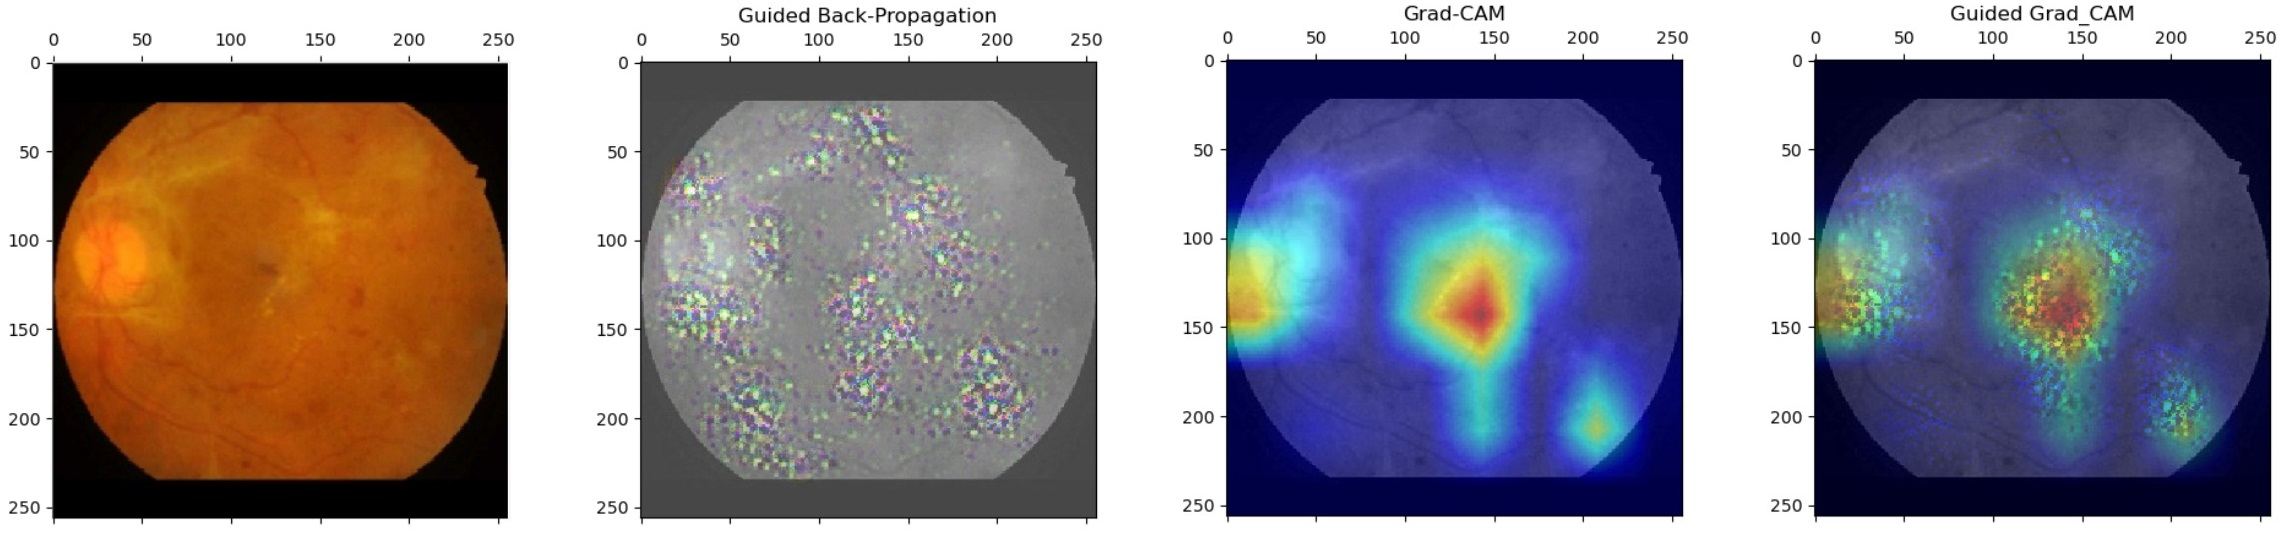
\includegraphics[scale=0.28]{../pictures/deep_visualisation/deep_visulisation.png}
%\caption{fig1}
}
\caption{Deep visulisation example for ResNet50}
\label{fig:fig4}
\end{figure}
Here we used the guided backpropagation, Grad-CAM, and their combination i.e. guided Grad-CAM to visualize our models. Figure \ref{fig:fig4} is the example of these approaches based on ResNet50. It's obvious to discover that the networks make decisions based on the detection of those symptoms like microaneurysms or exudates.



\subsection{Multiclass classification and hyperparameter tuning (Jonas Vogt)}



Best 4 Hyperparameter configurations on Vision Transformer 16 on multi-class classification task after tuning with Weights\&Biases are as in Table \ref{tab:table2}. Note that the SGD we used here is trained with a self-build cosine annealing schedule with the warm-up, and the dropout rate is the maximum rate of the linearly increasing dropout rates of different Transformer-encoder blocks. Figure \ref{fig:fig5} and Table \ref{tab:table3} show the confusion matrix and matrices correspond to the model with the best performance.

If you want to read our tuning with Weights\&Biases in detail, please turn to our sweep report: 
\begin{center}
\url{https://wandb.ai/yitianshi/HP_VIT16/reports/Parameter-tuning-for-vision-transformer-16--VmlldzoxNTMxODAz}
\end{center}


\begin{table}
 \caption{Results of top 4 accuracy from hyperparameter tuning with Weights\&Biases}
  \centering
\begin{tabular}{ccccc}
\toprule
optimizer	&dropout rate&	learning rate	&weight decay	&test accuracy\\
\midrule
Adam&	0.0	&1.6e-3	&2.4-4	&61.17\%\\
SGD (with cosine annealing)&	0.1	&1.6e-2\footnote{}	&5e-4	&60.19\%\\
Adam&	0.1	&1.1e-3	&3.1e-4	&60.19\%\\
Adam&	0.2	&1.5e-3	&2.1e-4	&60.19\%\\

   \bottomrule
\
\label{tab:table2}
\end{tabular}
\end{table}

\begin{table}
\centering
\caption{Metrices}
\begin{tabular}{ccccccc}
\toprule
class against all&	Sensitivity	&Specificity	&Precision	&Accuracy	&Balanced-accuracy	&F1 score\\
\midrule
0	&88.24\%	&81.16\%&	69.77\%&	83.50\%&	84.70\%&	77.92\%\\
1	&0.00\%	&97.96\%	&0.00\%	&93.20\%&	48.98\%&	0.00\%\\
2	&68.75\%	&74.65\%	&55.00\%	&72.82\%&	71.70\%&	61.11\%\\
3	&42.11\%	&92.86\%	&57.14\%	&83.50\%&	67.48\%	&48.48\%\\
4	&23.08\%	&98.89\%	&75.00\%	&89.32\%&	60.98\%&	35.29\%\\
   \bottomrule
\
\label{tab:table3}
\end{tabular}
\end{table}



\begin{figure}
\centering
{
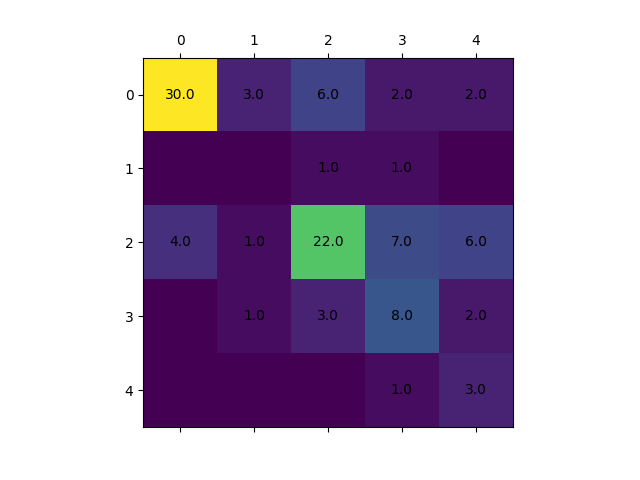
\includegraphics[scale=0.53]{../pictures/5-class classification for vit-16.png}
%\caption{fig1}
}
\caption{Confusion matrices of 5-class classification for ViT-16}
\label{fig:fig5}
\end{figure}

\footnotetext{Learning rate of the SGD is the maximum learning rate of the cosine annealing schedule}
\section{Conclusions}
\label{sec:conclusion}
After all, we've tried various model structures no matter if they were based on transfer learning or not. The Graham preprocessing seems not always better than the normal dataset under the condition of insufficient data. Moreover, although the models pretrained on ImageNet-21k show faster convergence during the training, since the source and target domains are quite dissimilar, the overall performance does not have any remarkable increase. However, there are only very limited reviews related to domain adaptation and their applications in medical image analysis which is a broad and important research area\cite{Hao}. 

Above all, the highest test accuracy we've achieved is 87.37\% for binary classification by hard voting and 61.17\% for 5-class classification. 
\subsection{First trial on Kaggle dataset (Yitian Shi)}
We've also built a pipeline to train the models based on the Kaggle dataset offered by the institute, which is already preprocessed by the Graham preprocessing. Since the computation resource is limited, the training of all the parameters for architectures such as the EfficientNet family is not feasible. What we can do here is just to fine-tune the last several layers of the pre-trained model based on the Imagenet-21k. We achieved a total accuracy of 71.17\% for EfficientNetB2 at first, but because of the huge unbalance of data, the balanced accuracy only reached 44.35\%. After applying balanced weights in the focal loss as our loss function, the balanced accuracy was increased to 49.71\%, but the total accuracy was reduced until 56.22\%. In summation, more GPU memory is expected to train a larger model for this dataset. 

\bibliographystyle{unsrt}  
%\bibliography{references}  %%% Remove comment to use the external .bib file (using bibtex).
%%% and comment out the ``thebibliography'' section.


%%% Comment out this section when you \bibliography{references} is enabled.
\begin{thebibliography}{1}



\bibitem{misgina}
Misgina Tsighe Hagos, Shri Kant
\newblock Transfer Learning based Detection of Diabetic Retinopathy from Small Dataset
\newblock {\em arXiv:1905.07203v2}, 2019.
\bibitem{Hao}
Hao Guan, Mingxia Liu
\newblock Domain Adaptation for Medical Image Analysis: A Survey
\newblock {\em 	arXiv:2102.09508}, 2021.

\end{thebibliography}

\end{document}

